\begin{figure}
  \begin{center}
    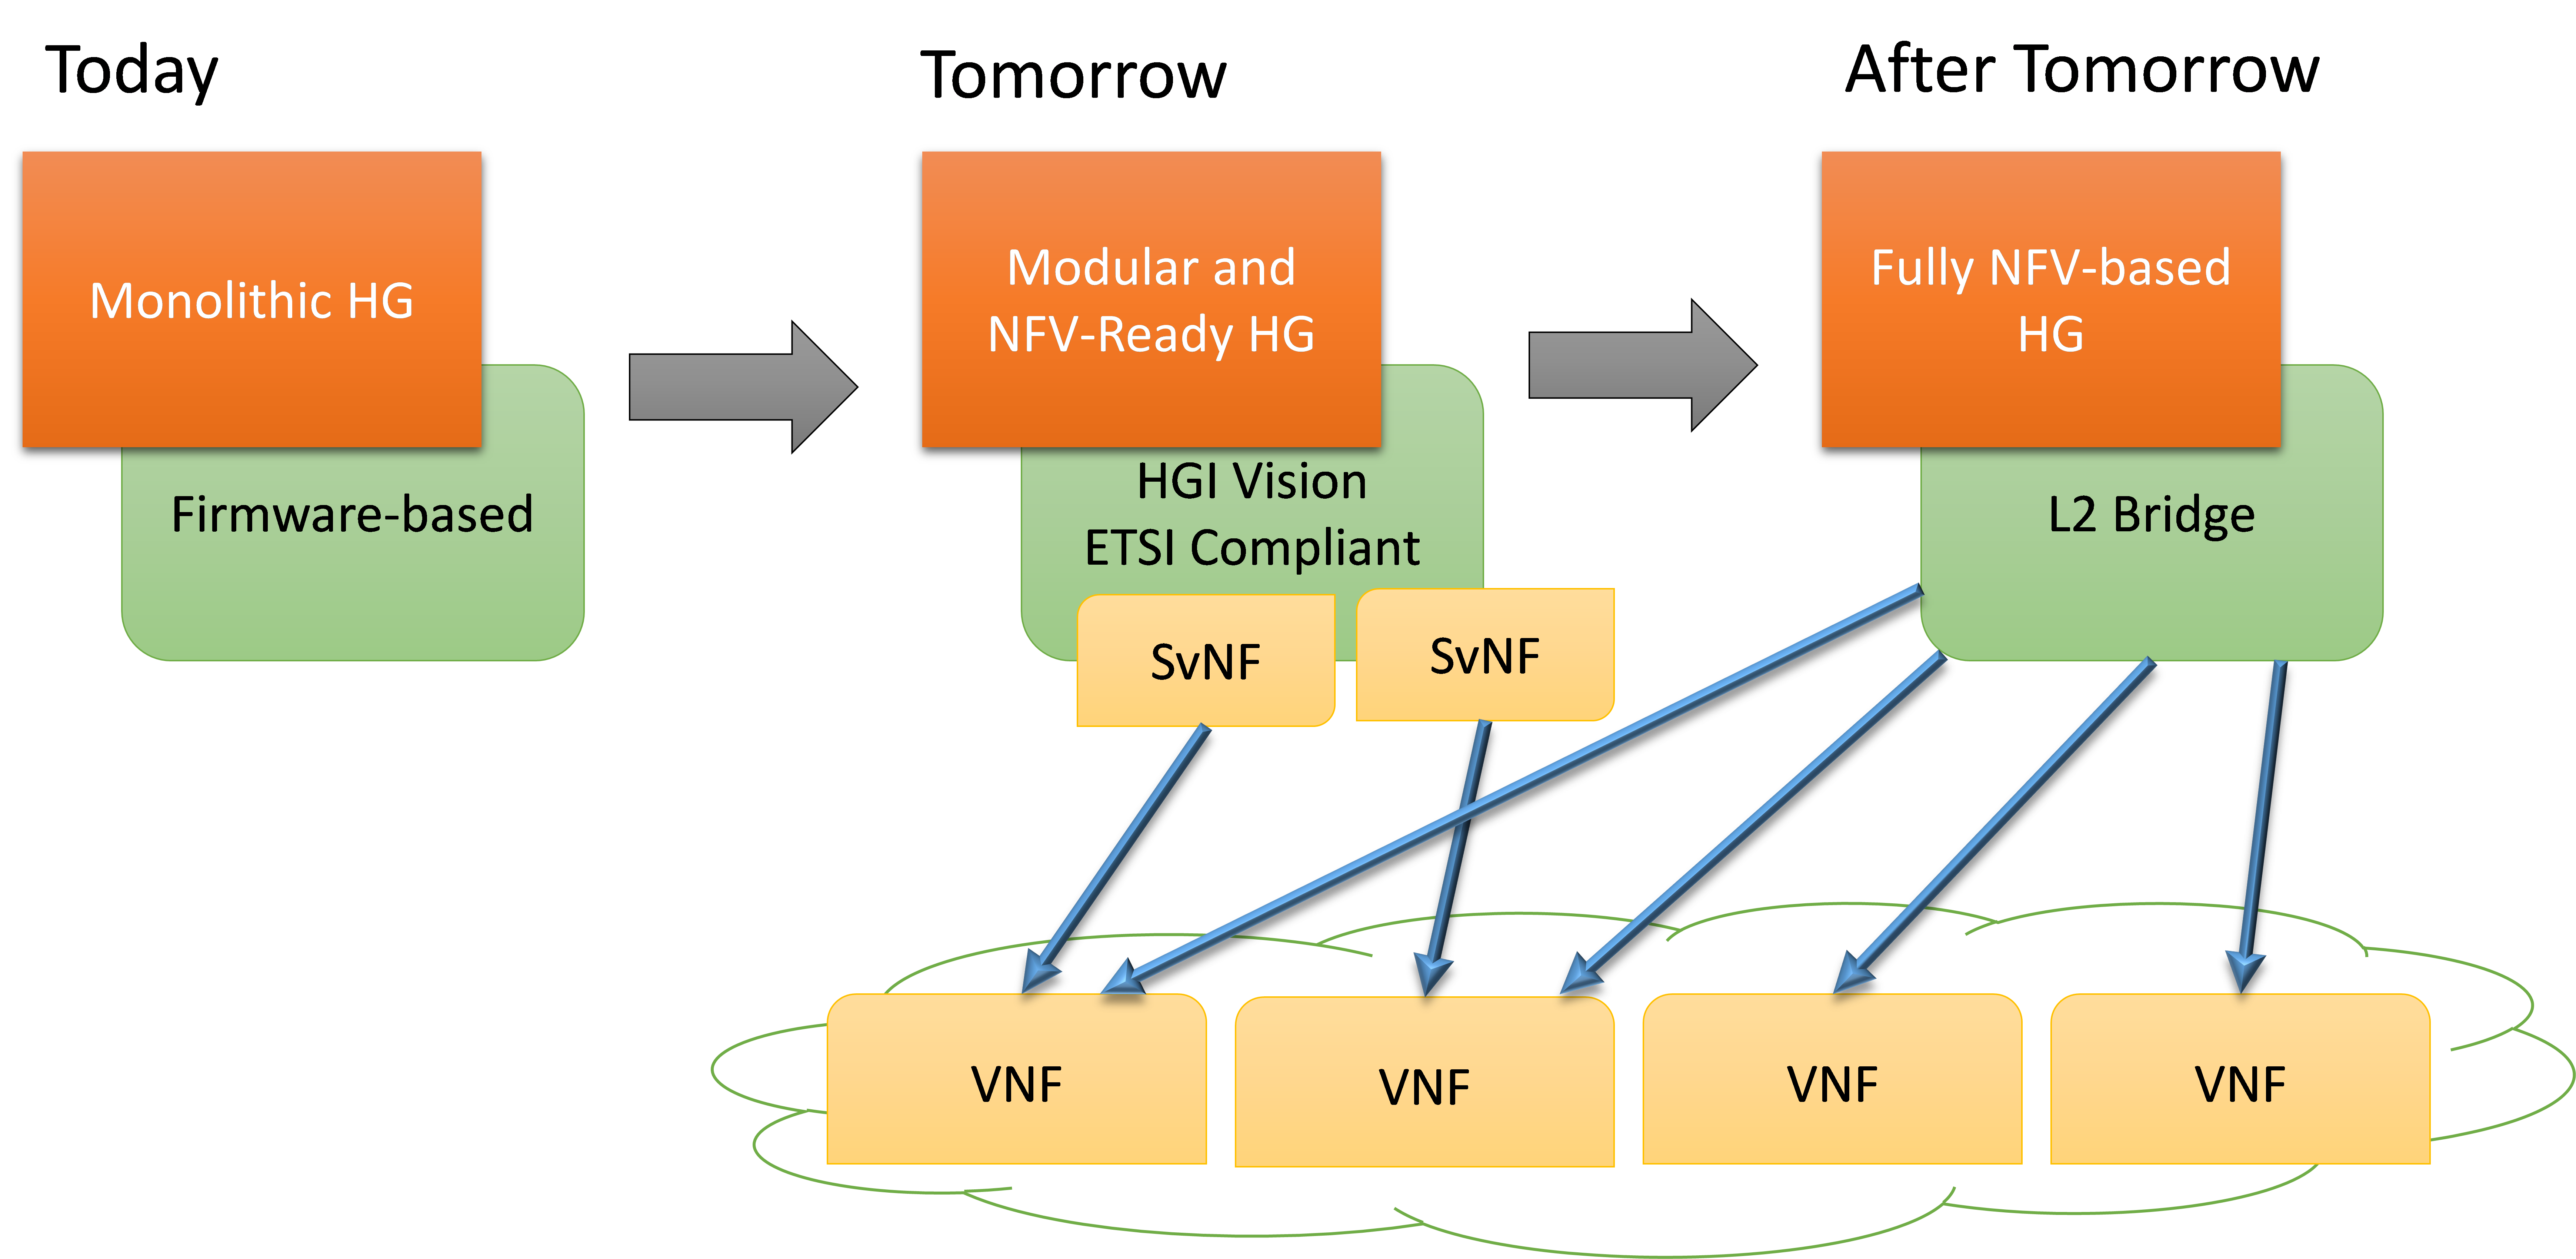
\includegraphics[width=0.45\textwidth,natwidth=6955,natheight=3398]{fig/vhgMigrationPath.png}
  \end{center}
  \caption{ Migration path from Modular to Virtual HG.
    \label{fig:migration}
  }
\end{figure}


\subsection{The NFV ready Modular HG}
We propose an alternative migration path where vNFs collaborate with modular gateways.
Figure~\ref{fig:migration} presents a Modular HG with \textit{"Surrogate vNF"} (SvNF) deployed on the device.
A SvNF is an OSGi bundle that acts like a regular module from the HG standpoint, except that it delegates any significant operation to a vNF.

SvNF modules can be aware of SP access network capabilities to support vNFs, so they can be registered in the HG OSGi execution environment only if they are supported by the underlying network.
For example, if the gateway cannot find any suitable vNF in a predefined SP point of presence (POP) list, it will fall back on legacy mode and keep using the native functionality instead of the virtualized one.

The key role played by the couple SvNF+vNF in the migration path is that the vNF part is used on both the OSGi modular gateway scenario and on the L2 bridge scenario.
This approach helps the SP stabilising its vNF before gradually migrating all its customers to the full vNF solution while securing investments made on developing the vNF.
 
\subsection{Concept and feasibility}
To demonstrate the feasibility of a modular and NFV-ready HG, we realized a proof of concept (POC).
In order for this POC to be highly relevant, we had to consider the best possible Network Functions to be virtualised.
We could have focused on simple functions such as DHCP or NAT but since they are not difficult tasks to be processed, the added-value of virtualizing them appears limited.
We thus decided to highlight the advantages of our proposal by deploying a new type of SvNF+vNF related to video distribution that would leverage the End-User's Quality of Experience related to video consumption and enhance network performances at the same time.
Such a function can be introduced into a modular OSGi HG and its execution would definitely be efficient as a vNF, due to the heavy video processing tasks it involves.
It is expected that IP video traffic will reach almost 80\% of all consumer Internet traffic in 2018 [CISCO forecast white paper: http://www.cisco.com/c/en/us/solutions/collateral/service-provider/ip-ngn-ip-next-generation-network/white_paper_c11-481360.html], therefore it seems important to focus on how new solutions, such as NFV, could not only cope with this but especially enhance the delivery of such data.

\begin{figure*}
	
	\center

	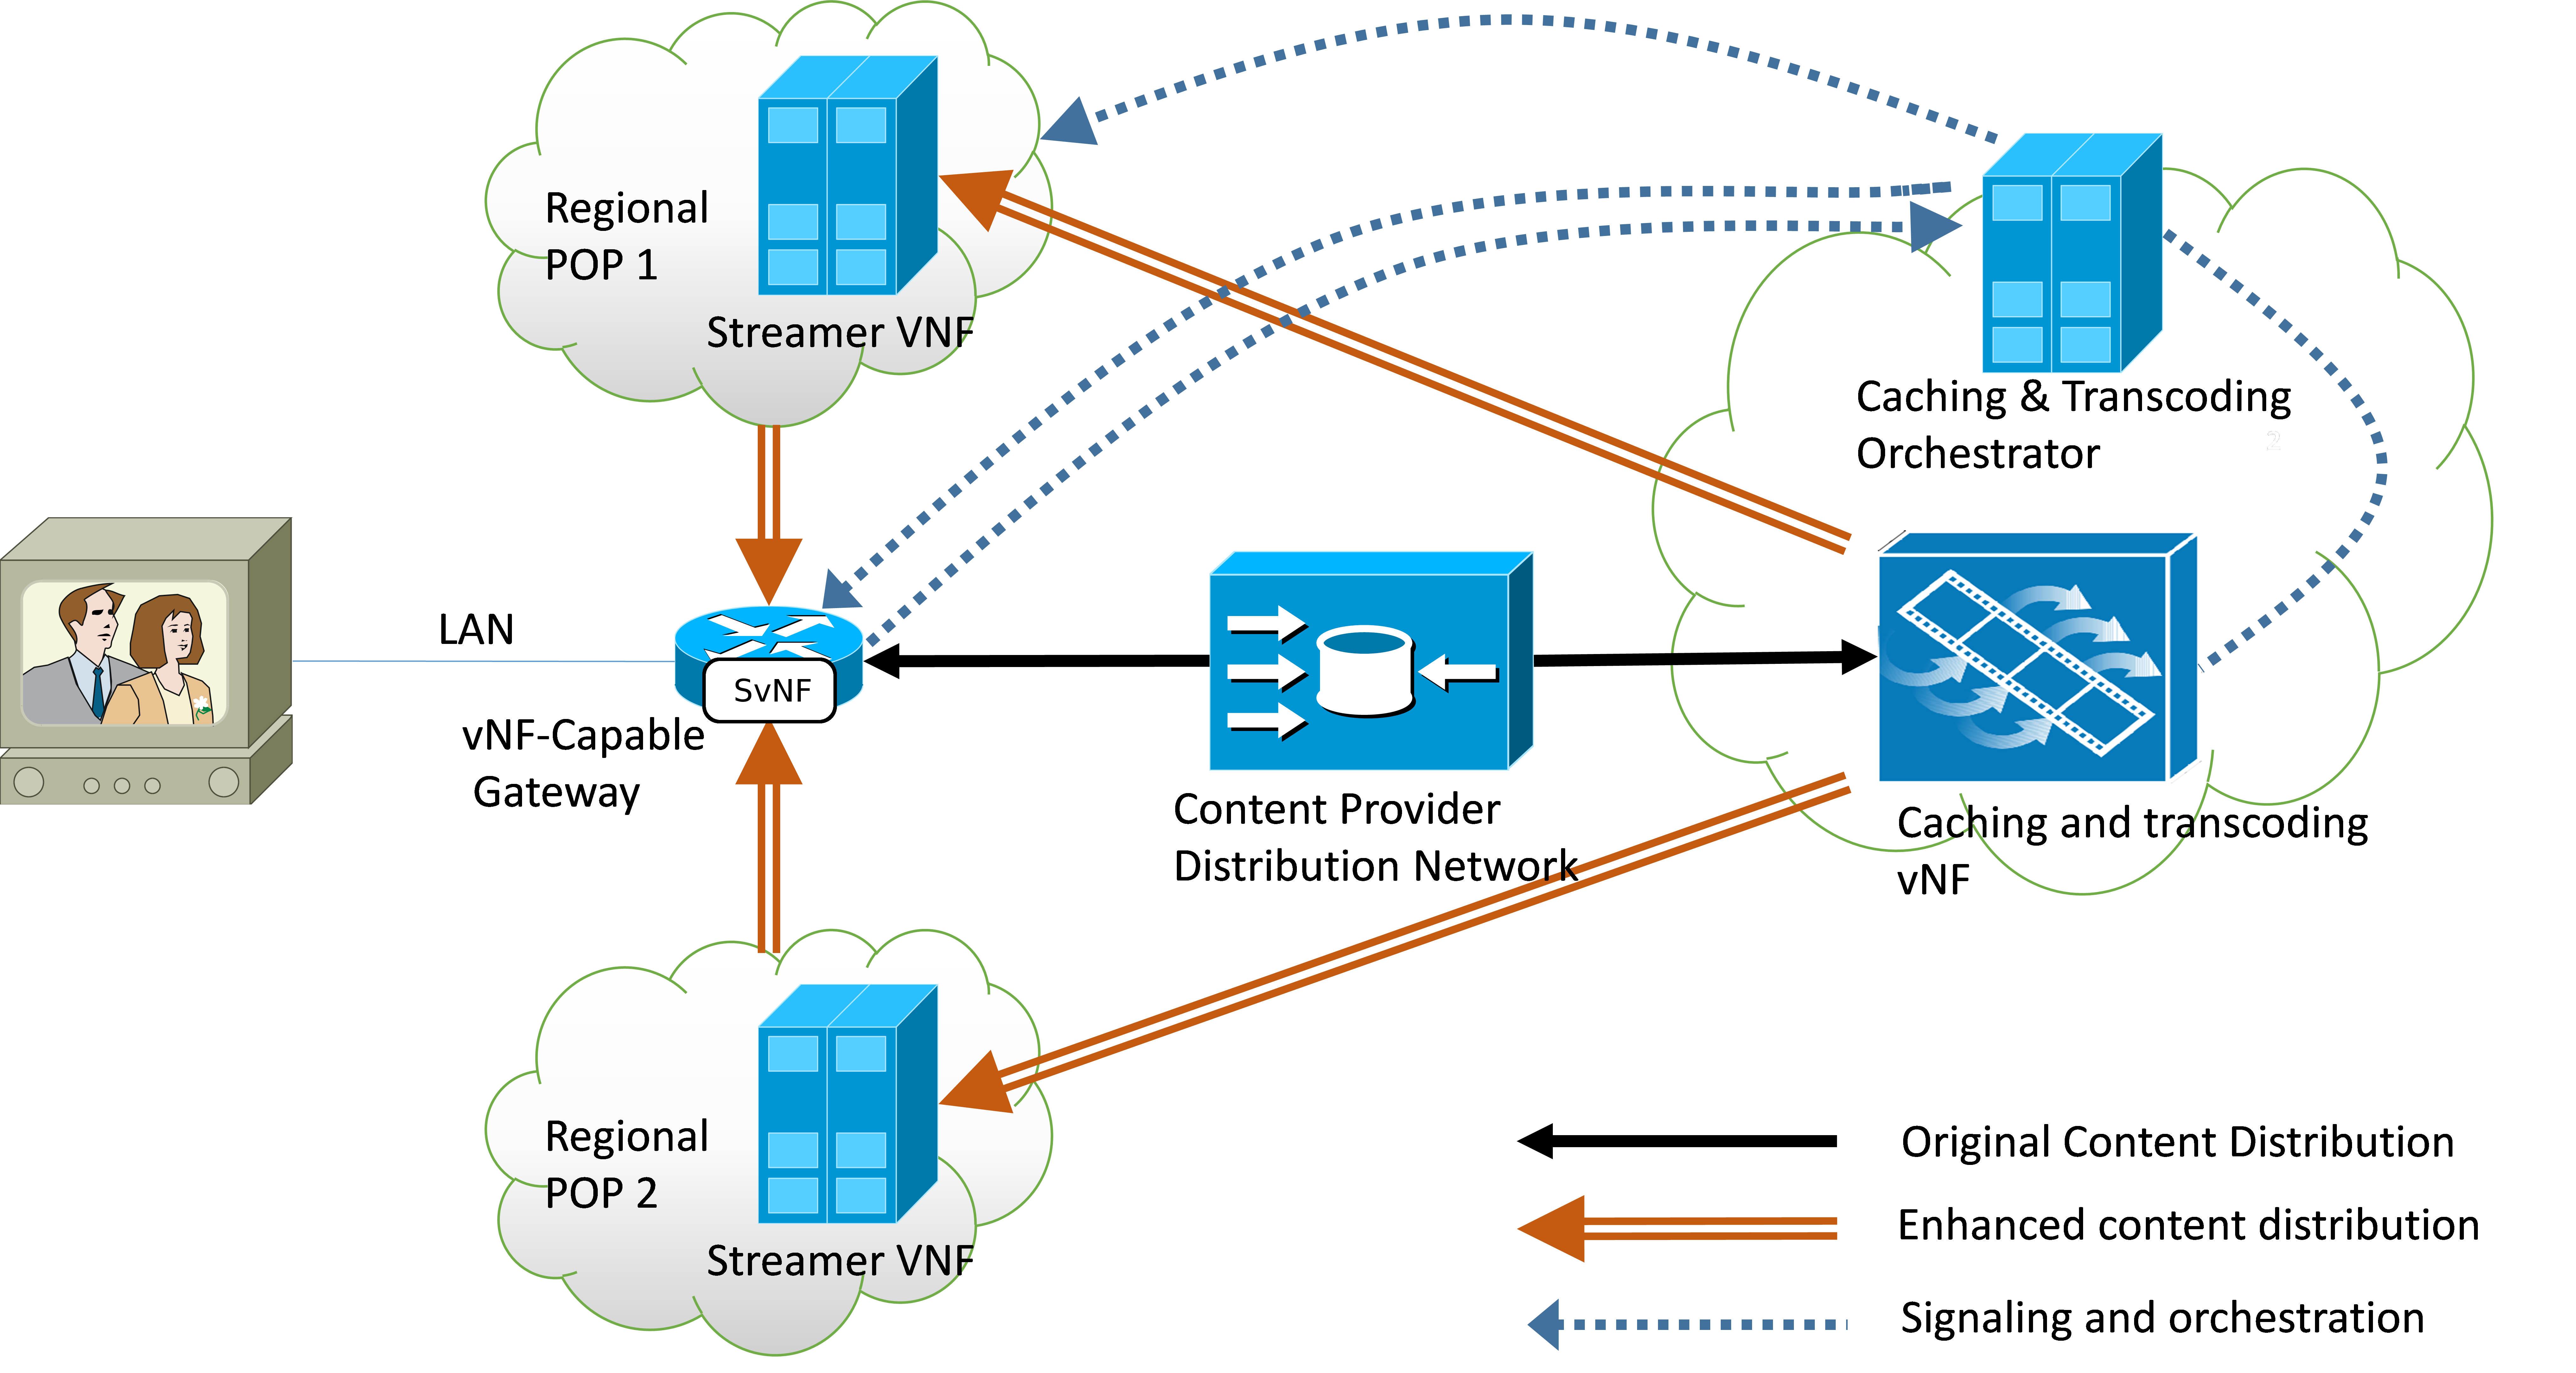
\includegraphics[width=0.90\textwidth,natwidth=8132,natheight=4335]{fig/highleveldesign.png}
	\caption{ High level design
    \label{fig:hld}
    }

\end{figure*}


The use case considered consists of an End User consuming media from his Set-Top Box, linked to his HG (the two devices are more and more often combined into one).
Video streams of a VOD or IPTV service are transferred from the content provider distribution network (which may or may not include Content Delivery Networks - CDNs) to the TV and cross the modular OSGi Gateway.
Figure~\ref{fig:hld} depicts the design of the system and the use case steps. 
   
The figure presents the interactions between CP, SP and EU for a classical video streaming use case.
In the original content distribution model, content is stream from the content provider network to the user gateway.
Classic deployment scenario involve the use of content distribution network to offload the CP main server.
CDN nodes are often collocated with internet exchange points (IXP) which present the advantage of being located relatively close of the EU.
Our use case however, presents an alternative model where the content is cached in regional POP managed by SP (also called micro-data centers located at the edge of the network) and exposed for streaming by a vNF.
Caching and encoding orchestrator manages configuration deployments of the SvNF on the gateways, the provisioning of regional POPs, as well as the caching and transcoding vNF.

The SvNF module deployed on the HG works as a HTTP proxy.
When it receives a request for a file or a response from a server, it analyses them using a set of rules deployed on the HG by the Caching and Transcoding Orchestrator through the "Caching Control and Configuration Channel".
Depending on the result several scenarios can occur.
Content could be available only in the CP network or an enhanced version could be cached by the system into a close regional POP.
Let's consider the three possible scenarios.
For the three possible scenario, the steps 1 and 2 are the same. 

\paragraph{Step1}EU requests the content from the vNF-Capable Gateway. 
\paragraph{Step 2}
The vNF-Capable Gateway analyses the video format, and checks it is technically compatible with the system (e.g. a supported video codec and supported delivery method).
If it is compatible, we continue to scenario 2, otherwise, we proceed with scenario 1.

\subsubsection*{Scenario 1: no operation scenario}

In this scenario, the content consumed by the user is not eligible to the enhancements brought by the system.
After the gateway has analysed the request, it if forwarded to its original destination.

\paragraph{Step 3}The content is then directly consumed by the End-User from the Content Provider Delivery Network.
This is the common case, as it is performed today.
The HG does not bring any added value to the consumption of video streams.
It just lets the content pass through it.

In this case, the SvNF creates an overhead on the gateway without bringing additional value to the user.
This overhead needs to be measured in order to know if it would penalize the user experience (and in which extent).

\subsubsection*{Scenario 2: Cache hit scenario}

Let's now consider that the content has been processed by the system and is made available in regional POPs.
Those are part of the NVF infrastructure, and handle mostly storage and delivery of content.
They are managed by SP and can be collocated with existing O-CDNs (operator-managed CDN).
The Caching and Transcoding Orchestrator has configured SvNF so that the HG redirects the user request to a Streamer vNF.
Hopefully, those vNFs are deployed in regional POPs and provisioned in a way that network performances are enhanced with respect to the original Content Provider network.
The main value compared with the CDN approach is that content has been processed by the system and a "better version" of it is made available to the user through QoE enhancing techniques we will describe latter in (reference).

We can also consider that by leveraging the existing SP network, the approach can provide POPs that are much closer from the EU than in the CDN scenario.
This is a great way for the CP to generate extra revenue from its network.	

\subsubsection*{Scenario 3: Cache miss scenario}

Finally, the last scenario is the one where the content is eligible for caching and transcoding but no cached version is yet available to the vHG from where the request has been made.
In this case the cache is missed and the content is retrieved from the CP.

If the content only resides on the CP distribution network, user request is left untouched and media is consumed from there.
However, under the hood, SvNF has analysed both request and response and has checked if media was eligible for caching and transcoding.
The decision is made taking into account several properties on the HTTP resources like server domain, file type, file size and any relevant HTTP headers.
When an eligible content is found, the SvNF informs the Caching and Transcoding Orchestrator by sending a caching request.
Caching and Transcoding Orchestrator takes the decision to perform caching and transcoding on the content based on several criteria ranging from Context and User Intelligence (which has been proven in \cite{wang_cpcdn:_2015} to improve the performance of content delivery), to business negotiation between Content Provider and service Provider.

If the Caching and Transcoding Orchestrator decides to process the content, it informs the Caching and Transcoding vNF which in turn is in charge of downloading the content from the content provider and processing the content.
Once processed, the Caching and Transcoding Orchestrator provision streamer vNF in regional POPs according to the demand.
We develop on the specific operations carried out by the Caching and Transcoding vNF in (reference).

Once the content is deployed in selected POPs, the configuration is published to vHGs, allowing future requests to be routed to vNF streamers.

Otherwise, if the content is already available in other POPs in the system, the caching and transcoding orchestrator may reconsider its provisionning decisions by deploying the content in additional POPs in order to match a certain SLA.
This operation should be carried out with the help of the underlying NFV platform, like the T-NOVA project.

\subsection{In-network processing benefits for CP and SP}
The NFV approach allows us to process data directly in the network.
For our use case, it means that we can apply arbitrary modification to a video with a view to optimize the delivery with respect to a specific technical or business objective.
For example, targeted ads can be added to the video by the SP with a view to increase profit, QOE can be increased by transcoding the content into a specific format which has this property.
The fact that we are able to transform the content directly into the network is a big advantage in term of flexibility and convenience of administration for CP and SP.

One other striking features of NFV is its ability to dynamically provision network functions according to simple business requirements expressed as Service Layer Agreements (SLA).
To fine-tune orchestration policy of the system, SP could set a target of 10Mps in the 7pm-10pm time slot for its user toward a specific VOD website.
Once the vNF is configured with those targets, Caching and Transcoding Orchestrator has to do its best to respect the SLA by using NFV infrastructure metrics (CPU, IO, Memory) but also specific application metrics.
Thanks to the key roles played by the HG, our solution offers the possibility to collect metrics at the user level and hence using a Collective Intelligence approach to optimize system operation according to SLA targets. 

Collective intelligence data is collected thanks to caching requests emitted by vHG.
The system gathers data which reflect video consumption patterns on a per-user basis, like user average bandwidth, hourly consumption patterns, and consumption habits.
Let's imagine a particular user watch HBO's Game of Thrones every Monday evening on his Ipad which support Apple's HTTP Live Streaming (HLS) on a T1 connection.
If this pattern is widespread amongst users, the Caching and Transcoding Orchestrator can assign a higher priority on the transcoding of the HD HLS version of the popular TV show and assuring the correct provisionning on selected regional POPs.

This approach allows CP to broadcast its content in cooperation with SP NVF network with limited technical interaction.
Indeed, expressing contractual SLA target is enough for the CP to deploy its content, as the SP's vNF becomes responsible for determining (1) which content to cache (2) which enhancements to bring to the content and (3) where to cache the content.
